\chapter{The Π-Ware library}
\label{chap:piware}

    Π-Ware is an \ac{EHDL} that allows for circuit description (modelling),
    simulation, reasoning (proving correctness or other properties), and synthesis to netlists.
    In this chapter we will describe in detail how the Π-Ware library is organized,
    what principles are behind some of the most important design decisions taken in its development,
    and how to use Π-Ware to model, simulate and reason about circuit behaviour.

    The reader is assumed to be familiar with the \emph{Agda} programming language,
    as this is the language in which Π-Ware is embedded.
    An introductory-level knowledge of dependent type theory in general is also appreciated.


    \section{Circuit Syntax}
    \label{sec:circuit-syntax}
        %% Shallow vs. deep embedding
        %% Structural modelling
        %%     Represent connections among circuits in the DSL, \emph{not in the metalanguage}
        %%     Avoid having to deal with observable sharing

        The most basic activity allowed by Π-Ware is the \emph{description} of circuits:
        as already mentioned briefly in the introduction, Π-Ware is \emph{deeply} embedded,
        which means there is a \emph{datatype} whose values are circuits.

        A deep embedding was chosen in order to allow for semantics other than execution (simulation).
        Particularly, the possibility of \emph{synthesizing} circuit models was a requirement
        kept in mind throughout the whole development.

        The circuit datatype (\AD{ℂ'}) is the most \emph{fundamental} of the whole library.
        It is defined as an dependent inductive family, indexed by two natural numbers,
        as shown in Listing~\ref{lst:Circuit-core}.

        \begin{listing}[h]
            \ExecuteMetaData[agda/latex/PiWare/Circuit/Core.tex]{Circuit-core}
            \caption{The core circuit type (\AD{ℂ'}) of Π-Ware. \label{lst:Circuit-core}}
        \end{listing}

        A \emph{structural representation} of a circuit is achieved by the constructors of \AD{ℂ'}.
        This is in stark contrast with the the description style used in the Lava family, for example.
        In Lava, the constructors of the circuit datatype represent solely logic (or arithmetic) gates,
        and metalanguage (Haskell) constructs such as application, tupling and local naming are
        used to represent sequencing, parallel composition, loops and sharing.
        In Π-Ware, on the other hand, explicit constructors represent these combinations,
        avoiding the need to implement some form of \emph{observable sharing}~\cite{gill-typesafe-observable-sharing}.

        The indices of \AD{ℂ'} represent, respectively, the \emph{size} of the circuit's input and output.
        This can be thought of as the number of "wires" entering (resp. leaving) that circuit.
        Notice that the representation of inputs and outputs used in \AD{ℂ'} is untyped and unstructured.
        However, there is another -- higher-level -- circuit datatype (\AD{ℂ}),
        which adds a layer of typing \emph{on top} of \AD{ℂ'},
        and constitutes the actual intended "interface" between the user (hardware designer) and Π-Ware.
        This abstraction layer will be discussed in more detail on Section~\ref{subsec:high-level-circuit}.

        To better understand the reasoning behind the design of the low-level \AD{ℂ'} datatype,
        its constructors can be considered to belong to one of three categories:

        \begin{description}
            \item[Fundamental:] These construct "predefined", or "atomic" circuits, with no sub-components.
                \begin{itemize}
                    \item \AI{Nil}: The \emph{empty circuit}. Performs no computation and has neither inputs nor outputs.
                        It is mainly useful as a "base case" when building large circuits with recursive definitions.
                    \item \AI{Gate}: Constructs a chosen circuit among those provided by a \emph{gate library}
                        passed as parameter to the \AM{Circuit} module.
                    \item \AI{Plug}: Constructs a "rewiring" circuit. Performs no computation,
                        but can be used to apply permutations, associativity and to duplicate or discard wires.
                \end{itemize}
            \item[Structural:] Represent ways in which smaller circuits can be interconnected to build a bigger one.
                \begin{itemize}
                    \item \AI{c₁ ⟫' c₂}: Sequential composition.
                        Given $c₁$ and $c₂$, connects the output of $c₁$ into the input of $c₂$.
                    \item \AI{c₁ |' c₂}: Parallel composition.
                        Splits the input into two parts, connected to $c₁$ and $c₂$,
                        and rejoins the outputs of $c₁$ and $c₂$ into a single output.
                    \item \AI{c₁ |+' c₂}: Tagged branching.
                        Based on the value of a \emph{tag} given in one of the input wires,
                        feed the remaining input wires into \emph{either} $c₁$ or $c₂$.
                \end{itemize}
            \item[Delay:]
                The \AI{DelayLoop} constructor belongs to a category of its own.
                Its purpose is to construct a state-holding circuit given a purely combinational circuit as argument.
        \end{description}

        These descriptions are just a rough summary of the \emph{synthesis semantics} of Π-Ware, that is,
        how each circuit constructor creates a netlist, given netlists as arguments.
        The precise \emph{definitions} of the synthesis semantics is given in Section~\ref{sec:circuit-semantics}.
        The same section also contains a detailed definition and explanation of a simulation semantics
        for Π-Ware circuits, both purely combinational and sequential ones.

        \subsection{Design discipline enforced by circuit constructors}
            The several constructors of \AD{ℂ'} "calculate" the port sizes of the circuits they construct,
            based on the sizes of the circuits given as arguments.
            These calculations implement \emph{structural well-formedness} rules for circuits.
            One example of such rule can be seen in the case of parallel composition:

            \begin{center}
                \begin{code}
                    \>[4]\AgdaInductiveConstructor{\_|'\_} \<[11]%
                    \>[11]\AgdaSymbol{:} \AgdaSymbol{∀} \AgdaSymbol{\{}\AgdaBound{i₁} \AgdaBound{o₁} \AgdaBound{i₂} \AgdaBound{o₂}\AgdaSymbol{\}} \<[30]%
                    \>[30]\AgdaSymbol{→} \AgdaDatatype{ℂ'} \AgdaBound{i₁} \AgdaBound{o₁} \AgdaSymbol{→} \AgdaDatatype{ℂ'} \AgdaBound{i₂} \AgdaBound{o₂} \AgdaSymbol{→} \AgdaDatatype{ℂ'} \AgdaSymbol{(}\AgdaBound{i₁} \AgdaPrimitive{+} \AgdaBound{i₂}\AgdaSymbol{)} \AgdaSymbol{(}\AgdaBound{o₁} \AgdaPrimitive{+} \AgdaBound{o₂}\AgdaSymbol{)}\<%
                \end{code}
            \end{center}

            In this case, the input (resp. output) size of the composed circuit equals the \emph{sum}
            of the input (resp. output) sizes of the constituent sub-circuits.
            Other such rules are also imposed by \AI{\_⟫'\_}, \AI{\_|+'\_} and \AI{Plug}.
            Together, all of them ensure:

            \begin{description}
                \item[No floating wires] Circuit sizes need to match in order for the usage of a constructor
                    to be type-correct. In particular, no circuit \emph{input} wires are ever left "disconnected".
                    Figure~\ref{fig:sequencing-floating} illustrates an example of a situation banned by the sizing rule present
                    in the type of \AI{\_⟫'\_}.

                    \begin{figure}[h]
                        \centering{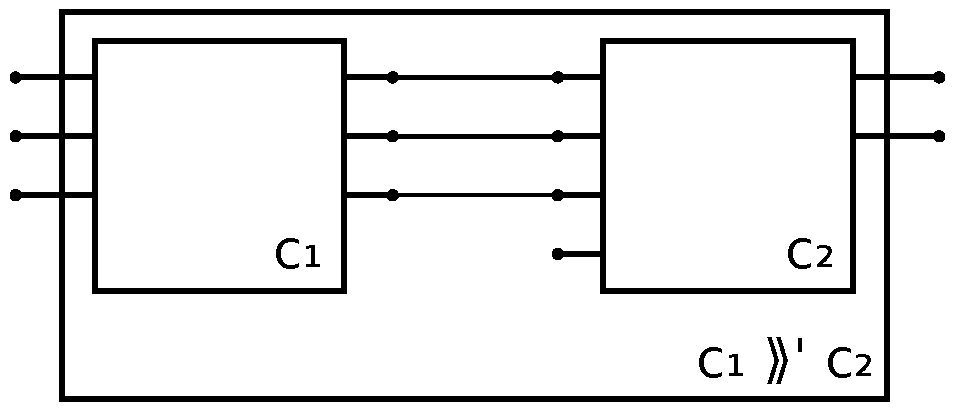
\includegraphics[width=0.6\textwidth]{imgs/sequencing-floating.pdf}}
                        \caption{Example of circuit banned by the type of \AI{\_⟫'\_}.\label{fig:sequencing-floating}}
                    \end{figure}

                \item [No short-circuits] The \AI{Plug} constructor, the only one which can be used for
                    "rewiring" purposes, has a type which forbids connecting multiple sources to the same load.
                    Its argument is a \emph{function from outputs to inputs}.
                    In this way, definitions connecting multiple inputs to the same output are banned,
                    as they are \emph{not} functions from outputs to inputs.
                    Also, when a plug is used between two sub-circuits $c₁$ and $c₂$,
                    a definition in which an \emph{input} of $c₂$ would be left "disconnected" is disallowed by Agda,
                    as such a definition would not be \emph{total}.
                    The diagram on Figure~\ref{fig:plug-seq-disconnected-input} represents such a banned situation:

                    \begin{figure}[h]
                        \centering{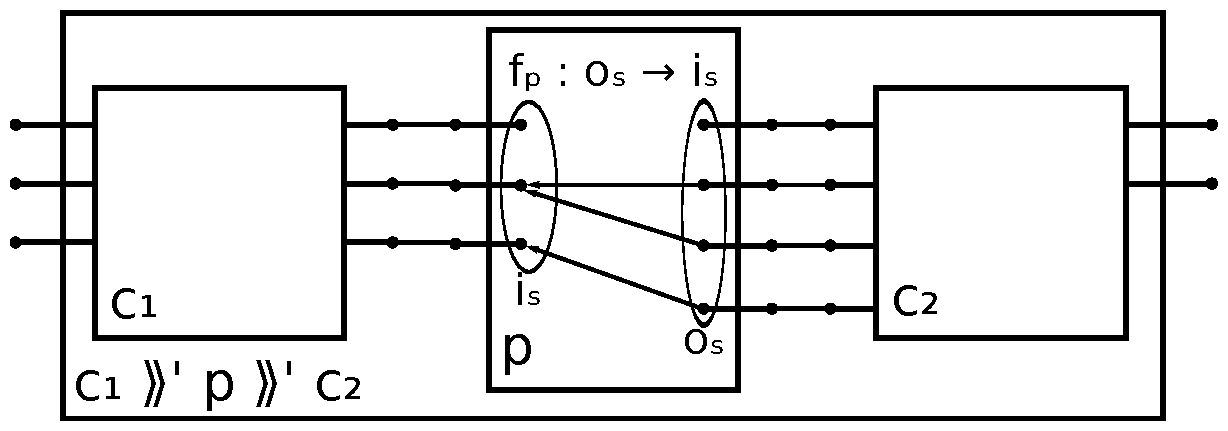
\includegraphics[width=0.8\textwidth]{imgs/plug-seq-disconnected-input.pdf}}
                        \caption{This circuit cannot be constructed because $f_{p}$ is not \emph{total}.\label{fig:plug-seq-disconnected-input}}
                    \end{figure}
            \end{description}

            \subsubsection{Purely combination vs. possibly sequential}
            Another piece of information "carried" together with circuits is whether it is
            \emph{purely combinational}, i.e., has no internal state, no notion of "history",
            and the value of its current outputs depend only on the value of its current inputs.

            This information is represented by a metalanguage truth value,
            an Agda \AF{Set} which can be either \AF{⊤} (the \AF{Set} with one value -- "top") or
            \AF{⊥} (the \AF{Set} with no values -- "bottom").

            The predicate \AF{comb'} over low-level (\AF{ℂ'}) circuits defines when is a circuit purely combinational.
            The code for \AF{comb'} is shown on Listing~\ref{lst:comb-core}.

            \begin{listing}[h]
                \ExecuteMetaData[agda/latex/PiWare/Circuit/Core.tex]{comb-core}
                \caption{Predicate telling whether a low-level circuit is purely combinational.\label{lst:comb-core}}
            \end{listing}

            Notice that the fundamental constructors \AI{Nil}, \AI{Gate} and \AI{Plug} \emph{always}
            build purely combinational circuits, while \AI{DelayLoop} always produces circuits with internal state.
            The structural constructors (\AI{\_⟫'\_}, \AI{\_|'\_} and \AI{\_|+'\_})
            yield a purely combinational circuit only when \emph{both} of its argument are themselves purely combinational.
            This is expressed by using the product type constructor \AF{\_×\_}, which in the \AF{Set}
            level corresponds to a logical conjunction.

            This categorization of circuits as stateful or stateless has one main goal:
            To avoid the evaluation of \emph{combinational loops}.
            Their presence in a circuit is almost always a design mistake, and by combining
            the \AI{DelayLoop} constructor with the \AF{comb'} predicate we guarantee that:

            \begin{itemize}
                \item The only way to create a loop in a circuit (\AI{DelayLoop}) also introduces a delay.
                \item Combinational evaluation (ignoring past inputs) only happens when safe.
            \end{itemize}


    \section{Abstraction Mechanisms}
    \label{sec:circuit-abstraction}
        Several of the definitions (modules, datatypes, functions) of Π-Ware are parameterized
        in order to provide for better code reuse.
        The library allows for a choice of the type of data carried in individual wires,
        the types that serve as inputs and ouputs to circuits,
        and the set of fundamental gates from which circuits are built.

        In this section we present how this flexibility is achieved,
        which requirements are imposed upon the parameters in each case of parameterization.
        Also, the motivation behind the chosen requirements is presented,
        based on the general goals of Π-Ware as well as the wish to impose as few constraints as possible.


        \subsection{Atoms}
        \label{subsec:atoms}
            In \acp{EDSL} of the current Lava family~\cite{observable-sharing-circuits},
            only values of type \mintinline{haskell}{Bool} and \mintinline{haskell}{Int}
            can be carried by the "wires", and circuits can only operate on inputs and outputs
            which are tuples or lists of these basic types.

            There is a little more flexibility in ForSyDe~\cite{forsyde1999},
            where the \mintinline{haskell}{ProcType} type class determines what values of what types
            can be used as inputs and outputs of \emph{process functions} (combinational circuits).
            ForSyDe has predefined instances of \mintinline{haskell}{ProcType} for fixed-width numeric types
            (\mintinline{haskell}{Int8}, \mintinline{haskell}{Int16}, etc.) and \mintinline{haskell}{Bool},
            while relying on \emph{Template Haskell} to generate instances for user-defined \emph{enumerations}
            at compile time.

            Π-Ware's approach is similar to ForSyDe's, in that it shares the same goal
            (to "carry" in the wires any type that belongs to a type class).
            However, Π-Ware does not use any metaprogramming, and uses dependent types
            to ensure that the provided instances satisfy desired properties.
            The type class \AD{Atomic} (shown in Listing~\ref{lst:atomic})
            expresses in Π-Ware what are the requirements for a type to be carried in the wires of a circuit.

            \begin{listing}[h]
                \centering{\ExecuteMetaData[agda/latex/PiWare/Atom.tex]{Atomic}}
                \caption{The \AD{Atomic} type class.\label{lst:atomic}}
            \end{listing}

            The fields \AL{Atom} and \AL{|Atom|-1} determine, respectively,
            the Agda \AD{Set} to be used as basis and \emph{how many elements} of this \AD{Set}
            are to be used as atoms (the number of atoms is actually \AF{|Atom|} \AY{=} \AI{suc} \AL{|Atom|-1}).

            Then there are the fields \AL{n→atom} and \AL{atom→n}, which define a \emph{bijection}
            between the \AL{Atom} type and \AD{Fin} \AB{|Atom|} (naturals from \AI{zero} to \AF{|Atom|}).
            Finally, the two last fields in \AF{Atomic} are proofs
            that \AL{n→atom} and \AL{atom→n} are inverses of each other,
            therefore proving that they are also bijections.

            \subsubsection{Instance for \texttt{Bool}}
            Included with Π-Ware there is already a predefined instance of \AD{Atomic} for \AD{Bool}
            (the boolean type in Agda's standard library).
            Knowing the meaning of each field, the definitions comprising the instance
            are mostly easy to understand.
            First, we start by defining the cardinality of the set of values we are interest in
            (\AD{B} is used as synonym for \AD{Bool}):

            \begin{center}
                \ExecuteMetaData[agda/latex/PiWare/Atom/Bool.tex]{cardinality}
            \end{center}

            Now, before defining the bijections that enumerate the set of atoms,
            we give more convenient \emph{names} to the elements of \AD{Fin} \AB{|B|} used in the enumeration
            by using an Agda feature known as \emph{pattern synonyms}:

            \begin{center}
                \ExecuteMetaData[agda/latex/PiWare/Atom/Bool.tex]{pattern-synonyms}
            \end{center}

            The usage of the \AI{Absurd\#} pattern becomes clearer when we take a look at
            the definitions of the bijections themselves:

            \begin{center}
                \ExecuteMetaData[agda/latex/PiWare/Atom/Bool.tex]{nToBool}
            \end{center}

            In the case of the \AI{Absurd\#} pattern, there is no need to provide a right-hand side
            to the equation, as the Agda typechecker can verify that
            there is no \AB{x} such that \AI{Fs} \AY{(}\AI{Fs} \AB{x}\AY{)} belongs to \AD{Fin} \AN{2}.

            Finally, there are the proofs stating that \AF{n→B} has a two-sided inverse (namely, \AF{B→n}),
            and, therefore, it is a bijection. The proofs use simple case analysis (and reflexivity).

            \begin{center}
                \ExecuteMetaData[agda/latex/PiWare/Atom/Bool.tex]{inv-Bool}
            \end{center}

            \subsubsection{Other possibly interesting instances}
            Even though currently \AD{Bool} (from the Agda standard library) is the only type for which
            there is already a predefined instance of \AD{Atomic}, other types could be interestingly used as atoms.
            For example:

            \begin{description}
                \item[Three-valued logic types]
                    Representing the values \texttt{TRUE}, \texttt{FALSE} and \texttt{UNKNOWN}
                \item[IEEE1164 nine-valued logic]
                    Standardized logic used widely in industry as a VHDL/Verilog type.
                    Besides the usual \texttt{FALSE} and \texttt{TRUE} logical values
                    (represented respectively by '0' and '1')
                    it accomodates also the following others:
                    \begin{itemize}
                        \item \texttt{'Z'}: \emph{High impedance}, means output is not being driven.
                        \item \texttt{'X'}: \emph{Strong drive, unknown logic value}.
                        \item \texttt{'W'}: \emph{Weak drive, unknown logic value}.
                        \item \texttt{'L'}: \emph{Weak drive, logic zero}.
                        \item \texttt{'H'}: \emph{Weak drive, logic one}.
                        \item \texttt{'U'}: \emph{Uninitialized}. Used as default initial value in simulation.
                        \item \texttt{'-'}: \emph{Don't care}.
                    \end{itemize}
            \end{description}


        \subsection{Gate library}
        \label{subsec:gate-library}
            Besides being parameterized by the type of \AD{Atom}s that can be carried in their wires,
            Π-Ware low-level circuit descriptions (\AD{ℂ'}) are also parameterized by
            a \emph{library of fundamental gates} upon which circuits are built.

            There are several interesting possible gate libraries which could be used to describe circuits,
            among which:

            \acrodef{DSP}{Digital Signal Processing}
            \begin{itemize}
                \item \emph{Functionally complete} sets of boolean functions such as
                    $\{ \text{\texttt{NAND}} \}$, $\{ \text{\texttt{NOR}} \}$ or
                    $\{ \text{\texttt{NOT}}, \text{\texttt{AND}}, \text{\texttt{OR}} \}$
                    (predefined in the Π-Ware library).
                \item Arithmetic primitives over boolean vectors, such as $\{ \text{\texttt{\_+\_}}, \text{\texttt{\_*\_}} \}$.
                \item A logic-arithmetic library together with some purpose-specific primitives,
                    for example cryptographic and \ac{DSP} functions.
            \end{itemize}

            A gate library is defined as an element of the \AD{Gates} record type, shown in Listing~\ref{lst:gates}.

            \begin{listing}[h]
                \ExecuteMetaData[agda/latex/PiWare/Synthesizable.tex]{Word}
                \newline
                \ExecuteMetaData[agda/latex/PiWare/Gates.tex]{Gates}
                \caption{Definition of a gate library: the \AD{Gates} record.\label{lst:gates}}
            \end{listing}

            The first field of the \AD{Gates} record (\AL{|Gates|-1}) determines \emph{how many}
            gates the library has, and consequently also the \emph{the type used as gate index}
            (or "gate identifier"), which is \AF{Gates\#} \AY{=} \AF{Fin} \AF{|Gates|}.

            For each gate identifier, the functions \AL{ins} and \AL{outs} determine, respectively,
            the size of the input and output of that gate; therefore together they determine the gate's \emph{interface}.

            Finally, the \AL{spec} field determines the \emph{functional specification} of a given gate identifier.
            Notice how the whole \AM{Gates} module is parameterized by an instance of \AD{Atomic}.
            In this way, the \AL{spec} function yields, given a gate identifier, a function over \emph{words}
            (\AD{Atom} vectors) of the correct length.
            This functional specification of each fundamental gate is used for the \emph{simulation semantics}.

            \subsubsection{Assumed correctness}
            Later, in Section~\ref{sec:proving-circuit-properties}, we will give a precise definition
            for what is considered the \emph{functional correctness} of a circuit; its \emph{compliance}
            to a certain functional specification.

            Usually, the proof of functional correctness for a circuit is built using, in some way,
            the correctness proofs of its subcomponents.
            However, fundamental gates have no subcomponents, so their correctness is assumed.
            By definition, the simulation semantics of a fundamental gate is equal to the \AL{spec}
            function given for it in the gate library definition.

            \subsubsection{Relation to synthesis}
            Even though fundamental gates are "atomic" (have no subcomponents) \emph{at the Π-Ware level},
            they are not in any way directly synthesizable to \ac{VHDL}.
            To convert a Π-Ware circuit to \ac{VHDL}, each fundamental gate in the library being used
            needs to have a corresponding excerpt of \ac{VHDL} code representing it.

            This feature is not integrated in the current version of Π-Ware, but assuming the existence
            of a hierarchy of datatypes representing \ac{VHDL} code, and specifically the existence
            of a type \AD{VHDLEntity}, we could have an extra field in the \AD{Gates} record, as such:

            \begin{center}
               \AL{netlist} \AY{:} \AY{(}\AB{g} \AY{:} \AD{Fin} \AY{(}\AI{suc} \AL{|Gates|-1}\AY{)}\AY{)} \AY{→} \AD{VHDLEntity} \AY{(}\AL{ins} \AB{g}\AY{)} \AY{(}\AL{out} \AB{g}\AY{)}
            \end{center}

            The \AD{VHDLEntity} is also parameterized by the input and output sizes of the circuit,
            tying the Π-Ware fundamental gate interface with the \ac{VHDL} abstract syntax.

            \subsubsection{Instance for \texttt{BoolTrio}}
            One specific instance of gate library is already "shipped" with Π-Ware:
            the usual set of boolean gates
            $\{ \text{\texttt{NOT}}, \text{\texttt{AND}}, \text{\texttt{OR}} \}$, together with
            the constants $\{ \text{\texttt{FALSE}}, \text{\texttt{TRUE}} \}$.
            The first definitions establish that this library contains five gates:

            \begin{center}
                \ExecuteMetaData[agda/latex/PiWare/Gates/BoolTrio.tex]{cardinality}
            \end{center}

            Then, as already done in the instance of \AD{Atomic}, we define some \emph{pattern synonyms}
            to make the gate identifiers easier to read:

            \begin{center}
                \ExecuteMetaData[agda/latex/PiWare/Gates/BoolTrio.tex]{pattern-synonyms}
            \end{center}

            The next step is to define the \emph{interface} of each gate on the library.
            All gates have exactly one output, while the number of inputs vary from 0 to 2.

            \begin{center}
                \ExecuteMetaData[agda/latex/PiWare/Gates/BoolTrio.tex]{ins-outs}
            \end{center}

            Finally, the last piece of information needed to define the gate library is
            the functional specification of each gate.

            \begin{center}
                \ExecuteMetaData[agda/latex/PiWare/Gates/BoolTrio.tex]{spec}
            \end{center}

            Notice that the gates use \AD{Bool} from Agda's standard library as their \AD{Atom} type.
            Also the logic operators from the standard library (\AM{Data.Bool}) are used in the specification.
            With all the necessary pieces of the puzzle in hand, the definition of the \AD{BoolTrio}
            gate library is as follows:

            \begin{center}
                \ExecuteMetaData[agda/latex/PiWare/Gates/BoolTrio.tex]{BoolTrio}
            \end{center}


        \subsection{High-level circuit datatype}
        \label{subsec:high-level-circuit}
            When presenting the low-level circuit datatype (\AD{ℂ'}) on Section~\ref{sec:circuit-syntax},
            it was mentioned that the representation using \AD{ℂ'} is untyped and unstructured, i.e.,
            all circuit inputs and outputs at that level are just sequences of \AD{Atom}s (for example, bits).

            However, the user of Π-Ware is not supposed to actually model circuits using the \AD{ℂ'} datatype.
            There is a layer of abstraction sitting on top of \AD{ℂ'},
            and circuits at this higher level have inputs and outputs with Agda types.
            This layer is coded as the \AD{ℂ} datatype, shown in Listing~\ref{lst:Circuit}.

            \begin{listing}[h]
                \ExecuteMetaData[agda/latex/PiWare/Circuit.tex]{Circuit}
                \caption{High-level circuit datatype (\AD{ℂ}).\label{lst:Circuit}}
            \end{listing}

            First of all, notice the \emph{lack of a prime symbol in the name of the datatype}.
            This is a general naming convention:
            whenever there are two versions of a definition, one at a low level of abstraction and one higher,
            the low-level gets the same name of the high-level one, with a prime symbol as suffix.

            In contrast to the low-level (\AD{ℂ'}) circuit type, \AD{ℂ} is parameterized by two Agda \AD{Set}s,
            and has only one constructor - \AI{Mkℂ} - which "packs" the low-level circuit description
            with the information on how to convert between the input/output Agda types
            (resp. \AB{α} and \AB{β}) and the appropriately-sized \emph{words} used in the low level.
            This conversion information is coded in the \AD{⇓𝕎⇑} type class (pronounced "Synthesizable"),
            which is covered in more detail on Section~\ref{subsec:synthesizable}.

            Furthermore, the \AM{PiWare.Circuit} module defines also \emph{smart constructors} for \AD{ℂ},
            corresponding to each of the constructors at the low level.
            One example is parallel composition:

            \begin{center}
                \ExecuteMetaData[agda/latex/PiWare/Circuit.tex]{par}
            \end{center}

            Using a \emph{gate library} together with these smart constructors, one can model
            hardware circuits operating over Agda types.
            One very simple example is a \texttt{XOR} circuit (shown in Listing~\ref{lst:xor-sample}),
            built using the \texttt{BoolTrio} gate library mentioned before.
            The block diagram in Figure~\ref{fig:xor-sample} illustrates the architecture of such circuit.

            \begin{figure}[h]
                \centering{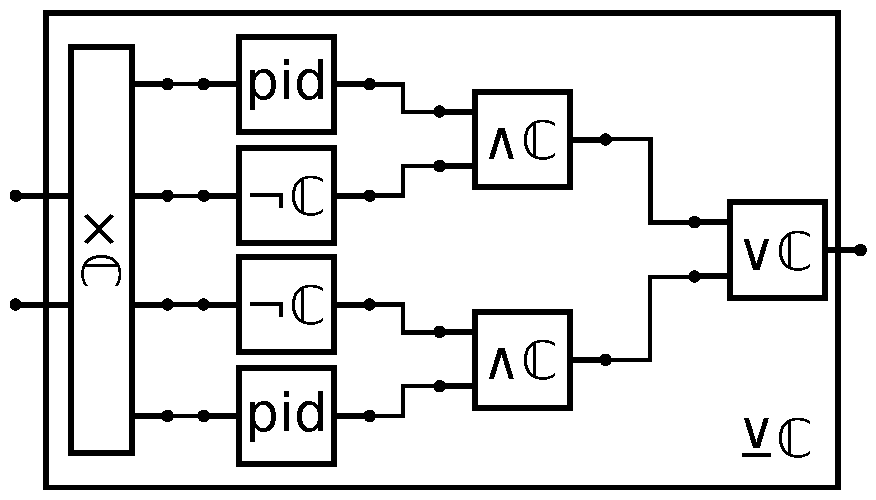
\includegraphics[width=0.50\textwidth]{imgs/xor-sample.pdf}}
                \caption{Architecture of a sample \texttt{XOR} gate.\label{fig:xor-sample}}
            \end{figure}

            \begin{listing}[h]
                \ExecuteMetaData[agda/latex/PiWare/Samples/BoolTrioComb.tex]{fundamentals}
                \newline
                \ExecuteMetaData[agda/latex/PiWare/Samples/BoolTrioComb.tex]{xor}
                \caption{Example of a \texttt{XOR} gate built with the \texttt{BoolTrio} library.\label{lst:xor-sample}}
            \end{listing}

            Again in this example, as customary, we renamed \AD{Bool} to \AD{B},
            and \AF{pid} is the \emph{identity plug}.
            The identity plug can be substituted in the netlist by a bus (with the adequate sizes),
            and is defined (together with other useful plugs) in the \AM{PiWare.Plugs} module.


        \subsection{The \texttt{Synthesizable} type class}
        \label{subsec:synthesizable}
            The "connection" between the low-level (\AD{ℂ'}) and high-level (\AD{ℂ}) circuit types
            is done by the \AD{⇓𝕎⇑} type class (pronounced "Synthesizable").
            Instances of the \AD{⇓𝕎⇑} class define a mapping between a given Agda type
            and an appropriately-sized \emph{word} type.
            Word types (\AD{𝕎} \AB{n}, for some \AB{n}) are \emph{synthesizable} to \ac{VHDL} vectors,
            thus the name of the class.
            Listing~\ref{lst:Synth} shows the definition of \AD{⇓𝕎⇑}:

            \begin{listing}[h]
                \ExecuteMetaData[agda/latex/PiWare/Synthesizable.tex]{Word}
                \newline
                \ExecuteMetaData[agda/latex/PiWare/Synthesizable.tex]{Synth}
                \caption{The \AD{⇓𝕎⇑} (Synthesizable) type class.\label{lst:Synth}}
            \end{listing}

            The type class has two parameters: the type which it encodes (\AB{α}),
            and the size of the \emph{word type} to which \AB{α} corresponds (\AB{i}).
            Notice that the size parameter is passed \emph{implicitly}, because in some occasions
            Agda might be able to automatically infer (by unification) this value.

            One can imagine that all \emph{finite types} (types with finitely many elements)
            can be made synthesizable under the definition of \AD{⇓𝕎⇑}, given a certain encoding scheme.
            We do not give a proof of this statement, but one way of doing it would be to translate
            Agda datatype definitions into a sum-of-products view and then use a standardized
            encoding scheme (for example, some form of \emph{Church encoding}).

            Π-Ware does \emph{not} provide facilities for mapping arbitrary Agda datatypes into
            a sum-of-products view (we believe this is the domain of a \emph{generic programming} library,
            not of a hardware \ac{EDSL}).
            However, Π-Ware \emph{does} provide predefined instances of \AD{⇓𝕎⇑} for units (\AD{⊤}),
            booleans (\AD{Bool}), products (\AD{\_×\_}), vectors (\AD{Vec}) and sums (\AD{\_⊎\_}),
            in order to facilitate working with complex types when modelling hardware.

            One interesting instance to look at is the one for Agda's standard library vectors (\AD{Vec}),
            shown in Listing~\ref{lst:Synth-Vec}.

            \begin{listing}[h]
                \ExecuteMetaData[agda/latex/PiWare/Synthesizable.tex]{Synth-Vec}
                \caption{Predefined instance of \AD{⇓𝕎⇑} for fixed-length vectors.\label{lst:Synth-Vec}}
            \end{listing}


    \section{Circuit Semantics}
    \label{sec:circuit-semantics}
        Functional semantics for simulation\ldots

        \begin{itemize}
            \item Two types of evaluation: combinational and sequential
            \item Combinational eval requires a proof that the circuit contains no loops
                \subitem Eval of a fundamental gate is just its \emph{definitional behaviour}

            \item For sequential circuits we use a \emph{causal stream semantics}
                \subitem Current output depends on the current input and (possibly) on the past inputs
                \subitem \emph{Different} than plain Stream functions

            \item There's also an eval function which allows the circuit to be viewed as function from Stream to Stream
        \end{itemize}

        \subsection{Combinational evaluation}
        \label{subsec:combinational-eval}

        \subsection{Sequential evaluation}
        \label{subsec:sequential-eval}
            Initially we tried to write a semantics yielding simply a function over streams.

            But this is not quite a good semantic model for a synchronous sequential circuits,
            as a stream function is allowed to "look into future values" in order to produce
            the output stream, while a sequential circuit can only use information about its past inputs
            when calculating the next output.

            Therefore, causal streams\ldots

            \subsubsection{Causal Streams}

    \section{Proving circuit properties}
    \label{sec:proving-circuit-properties}
